\section{Metriken}
Um die nun implementierte Technik zu evaluieren, müssen die im dritten Kapitel genannten Metriken genauer analysiert werden. Deswegen soll ein Blick in verwandte Arbeiten der letzten Jahre Hinweise darauf geben, wie diese Metriken in anderen Arbeiten quantifiziert wurden und ob bzw. wie eine ähnliche Vorgehensweise in unserem Fall angewendet werden kann.

\subsection{Bearbeitungszeit}
Selbstverständlich ist die Effizienz ein Kriterium, welches implizit in jeder Arbeit berücksichtigt wird, da eine schnelle und effektive Navigation immer ein wichtiges Ziel einer jeden Technik ist. Wenn dies überhaupt explizit gemessen wurde, wurde dies in den meisten Fällen schlicht und einfach mit der Bearbeitungszeit erfasst, welche gegen die einer ähnlichen Technik verglichen wurde (z.B. bei \cite{Suma2010EvaluationEnvironments}, \cite{Kopper2006DesignEnvironments}, \cite{3_Pierce1997}, \cite{Wingrave2006OvercomingWIM}). 
Bei Pierce et al. \cite{3_Pierce1997} liegt der Schwerpunkt vor allem anderen auf diesem Punkt. So wird hier begründet, dass die Durchführungszeit auch andere Metriken parallel mit abfragt:

\begin{addmargin}[25pt]{0pt} 

\textit{“In addition, travel time indirectly measures how easily users of a technique can maintain their orientation, form and execute plans, and detect destination.”}\cite{3_Pierce1997}

\end{addmargin}

Doch bei der Entwicklung dieser Technik stellen sich zwei Problematiken, denn zum einen gibt es keine Technik, gegen die verglichen werden kann, zum anderen kann die Kommunikation zwischen Gruppenmitgliedern die resultierende Bearbeitungszeit negativ beeinflussen, obwohl sie ein Indikator für eine gut abgestimmte Reiseplanung sein kann.

Die Herangehensweise soll in diesem Fall also eine andere sein:
Die Platzierung der Nutzerplattform in der WIM ist ein typisches Beispiel für eine manuelle Zielerfassung deren Parameter von Fitts Gesetz beschrieben wird \cite{fitts1954information}.
Die Anwendbarkeit seines Modells auf zwei- und dreidimensionale virtuelle Umgebungen wurde in unzähligen Folgestudien nachgewiesen (\cite{mackenzie1992fitts}, \cite{drewes2010only}, \cite{zhai2004characterizing} für einen Überblick der Forschung).

Fitts' Gesetz beschreibt die lineare Abhängigkeit der benötigten Zeit (MT) von einem
Schwierigkeitsindex (ID), der sich wiederum aus der Zielentfernung (D) und Zielgröße (W) ableiten lässt ($ID=log_2(2D/W)$).

Fitts testete Schwierigkeitsindizes zwischen 1 und 10. Seine Teilnehmer benötigten dafür je nach Schwierigkeit zwischen 180 und 1100 ms \cite{fitts1954information}. An Computerarbeitsplätzen ist die Effizienz der Zielbewegungen typischerweise etwas schlechter (z.B. \cite{Forlines}, \cite{mackenzie1992fitts}, \cite{MacKenzie:2008:FTS:1357054.1357308}, \cite{Wobbrock:2008:EMP:1357054.1357306}), vor 
allem im Falle von 3D Zielbewegungen in virtuellen Umgebungen in denen kein taktiles Feedback verfügbar ist (z.B. \cite{arsenault2004importance}, \cite{grossman2004pointing}, \cite{teather2011pointing}, \cite{lubos2014analysis}).

Basierend auf den oben erwähnten Forschungsergebnissen entschieden wir
uns, dass der maximale Schwierigkeitsindex (ID) der motorischen
Interaktionsbewegungen bei der Nutzung unserer Technik nicht höher als fünf sein sollte, um Ineffizienz und Frustration zu vermeiden. Offenbar benötigen Nutzer auch für 3D Selektionsaufgaben mit etwas geringeren IDs schon etwa zwei Sekunden ( vgl. \cite{grossman2004pointing}, \cite{teather2011pointing}, \cite{lubos2014analysis}). Im Zusammenhang mit einer Zielentfernung von einem Meter, was in etwa der Distanz, die man angenehm durch Ausstrecken des Armes erreichen kann entspricht, ergibt sich daraus eine minimale Zielgröße von etwa 5 bis 6 cm. Dies wiederum entspricht bei der gewählten Skalierung (1:100) der WIM einer Genauigkeit von (+/-) 2,5 bis 3,0 Metern. Der rein motorische Zeitaufwand dafür sollte im Bereich von etwas über zwei Sekunden liegen.



\subsection{Genauigkeit}
Die Genauigkeit ist stets mit der resultierenden Distanz zwischen Position des Nutzers nach der Navigation und eines im Vorhinein festgelegten Ziels zu bestimmen. 
Explizit wird dies beispielsweise in \cite{Krekhov2018GulliVR} abgefragt: Bei der \textit{“Aiming”} genannten Technik soll der Nutzer in einem Zielgebiet landen, welches durch eine farbige Zielscheibe gekennzeichnet ist. Die durchschnittliche Distanz zum Bullauge ist dabei das Maß, welches die Genauigkeit bestimmt.
Wichtig zu erwähnen ist, dass die Genauigkeit in den meisten Fällen mit der Bearbeitungszeit zusammenhängt: Hat man mehr Zeit oder nimmt man sie sich, so ist in den meisten Fällen die Genauigkeit größer (vgl. dazu auch vorheriger Unterpunkt!).
So wird in manchen Arbeiten (\cite{BowmanTestbedTechniques}, \cite{3_Pierce1997}) eine bestimmte Genauigkeit vorausgesetzt, in dem man sich innerhalb eines bestimmten Radius zum Ziel befinden muss, damit die Reise als abgeschlossen zählt.
Die Genauigkeit so exakt zu quantifizieren ist in unseren Augen allerdings nicht zwangsläufig notwendig. 
Viel wichtiger, als möglichst nahe an einem vorher festgelegten Punkt zu landen, ist unserer Meinung nach, dass das gewünschte Ziel für alle Nutzer vollständig sichtbar ist. 
Deshalb erhalten die Nutzer in unserer Studie Bilder von Objekten, die sich in der zu bereisenden Umgebung befinden, welche sie so ansteuern müssen, dass alle Details auf dem Bild auch in ihrer Perspektive zu sehen sind.

Ein weiteres Kriterium, mit dem die Genauigkeit ebenfalls gemessen werden kann ist die Häufigkeit von Kollisionen mit der virtuellen Umgebung(vgl. \cite{Suma2010EvaluationEnvironments}). Unsere Technik bietet die Möglichkeit, die Nutzerplattform so zu platzieren, dass Kollisionen im Vorhinein vermieden werden. Dies liegt jedoch im Verantwortungsbereich des Nutzers und kann in engen virtuellen Umgebungen sehr umständlich sein. Eine zukünftige Weiterentwicklung der Technik wäre daher eine automatische Kollisionsvermeidung, die eine gewählte Plattformposition nachjustiert.


\subsection{Informationsaufnahme}
Mit der Aufnahme von Informationen beschäftigen sich Suma et al. \cite{Suma2010EvaluationEnvironments}. Sie schlagen dabei verschiedene Möglichkeiten vor:


\textbf{Objekterkennung:}\\
Der Nutzer erhält eine Liste von 36 Objekten, von denen er die Hälfte auf seiner Reise sehen konnte. Die andere Hälfte war nicht in der virtuellen Umgebung platziert. Er erhält acht Minuten Zeit, die Objekte mit \glqq War in der Umgebung\grqq{} und \glqq War nicht in der Umgebung\grqq{} zu klassifizieren. In der Evaluierung werden die \textit{False Positives} werden von den \textit{Correct True Positives} abgezogen und es ergibt sich somit ein Score von 0 - 18.


\textbf{Objektplatzierung:}\\
Der Nutzer erhält eine Karte der von ihm bereisten Umgebung sowie eine nummerierte Liste mit allen 18 Objekten, die in der Umgebung platziert waren. 
Er wird gebeten, die Nummer aller Objekte an der Stelle in der Karte einzutragen, an der er sie gesehen hat (oder gemeint gesehen zu haben).
Das Ergebnis wird im Folgenden von einer Drittperson geprüft und bewertet.
Dabei wird jedes richtig platzierte Objekt mit einem Punkt gewertet und es ergibt sich auch hier ein Score von 0 - 18. 

Die Objekterkennung wird in unserem Fall nicht abgefragt, da die Nutzer nur Teile der Karte bereisen und sich dabei auf das Finden der Bilder konzentrieren, sodass der Fokus auf einem anderen Task liegt und etwaige Objekte übersehen werden können.
Die Objektplatzierung allerdings wird auch in unserem Fall vorgenommen. Dabei werden den Nutzern, nachdem sie die Karte bereist haben und alle Bilder gefunden haben, diese Bilder erneut ausgehändigt, sowie eine Karte, die nur die Umrisse der bebauten \glqq Inseln \grqq{} sowie die Kirche als Orientierungspunkt zeigt.
In dieser sollen die Nutzer dann die Bildnummern, sowie die Blickrichtung in Form eines Pfeils einzeichnen.


\subsection{Nutzerkomfort}
Um den Nutzerkomfort zu messen, wird neben generellen Fragen zum Wohlbefinden in der Mehrzahl aller Arbeiten (z.B. \cite{Krekhov2018GulliVR}, \cite{Suma2010EvaluationEnvironments}, \cite{Usoh1999WalkingEnvironments}) der Simulator Sickness Questionnaire genutzt \cite{Kennedy1993SimulatorSickness}. Dieser fragt das generelle Wohlbefinden nach dem Aufenthalt in einer Simulation bzw. in unserem Fall nach der Navigation in einer Simulation ab.

Auch in unserem Fall soll die Technik so entwickelt werden, dass durch sie keine merkliche Verschlechterung des allgemeinen Wohlbefindens der Nutzer eintritt. Dieses wird durch das Durchführen des SSQ vor und nach jedem Durchlauf der Studie ermittelt, wobei sich der Wert nicht oder kaum  verschlechtern dürfte, da unsere Technik wie bereits beschrieben mit einem Minimum an Steering und Motionflow auskommt.

\subsection{Raumwahrnehmung}
Die Raumwahrnehmung der Nutzer wird häufig (z.B. \cite{Kopper2006DesignEnvironments}, \cite{Richardson1999}) abgefragt, indem der Nutzer die Himmelsrichtung zu einem anderen, schon bekannten Ort anzeigen muss. Hierfür wird der angezeigte Winkel von dem tatsächlichen Winkel subtrahiert, um die tatsächliche Abweichung zu bestimmen (“Pointing error”). \cite{Kopper2006DesignEnvironments} beschreibt dies anders als nach Bowmans Metriken als “Accuracy”.
In der Arbeit von Vuong \cite{29_POINTING_ERROR_jennyVuong_small}, S.23 werden aus verschiedenen Studien in virtuellen Umgebungen solche resultierenden Abweichungen zusammengefasst. Die meisten dieser Abweichungen liegen im Gebiet von 10 bis 40 Grad.
Ein Beispiel davon ist die Arbeit von Thorndyke et al. \cite{Thorndyke1980LNAVIGATION}, in welcher ein Experiment durchgeführt wird, in dem Testpersonen sich eine Umgebung durch Navigieren oder dem Lernen einer Karte merken sollen und dieses Wissen im Folgenden abgefragt wurde.
Die (in diesem Fall nicht virtuelle) Umgebung ist dabei ein Stockwerk eines Gebäudes. Die Testpersonen wurden in zwei Gruppen aufgeteilt: Diejenigen, die die Karte des Stockwerks intensiv (bis sie  lernen und diejenigen, die das Stockwerk durch Navigieren in diesem gelernt haben, da sie unterschiedliche Zeitdauer dort gearbeitet haben ( “1 to 2 months, 6 to 12 months, or 12 to 24 months”).
In verschiedenen Experimenten mussten sie u.a. die Richtungen anderer Räume anzeigen.
Die Ergebnisse dabei sahen wie folgt aus: 
\begin{addmargin}[25pt]{0pt} 

\textit{Map learner: $\approx 39 ^\circ$ \\
1-2 months experience: $\approx  25 ^\circ$ \\
6-12 months experience: $\approx  24 ^\circ$ \\
12-24 months experience: $\approx  19 ^\circ$ \\}
\end{addmargin}

Weißker \cite{Weibker2018SpatialEnvironments} vergleicht in seiner Arbeit die Abweichungen die durch Steering und Teleportations Navigation entstehen. In diesem Falle liegen die Abweichungen im Durchschnitt knapp unter 20 Grad.

Auch nach dem Nutzen unserer Technik sollen die Testpersonen eine Vorstellung der Umgebung haben, welche sie bereisen. Dies soll abgefragt werden, in dem die Nutzer nach jeder Reise die Richtung anzeigen, in der sie den zuletzt besuchten POI (also das letzte Bild) vermuten. Wie oben beschrieben wird daraus die Abweichung in Grad berechnet. 
Die Ergebnisse von Thorndyke und Weißker legen nahe, dass die durchschnittliche Abweichung zwischen 20 und 40 Grad liegen wird. Das Ziel der Technik wird also sein, diesen Wert möglichst nahe an 20 Grad anzunähern und einen Wert von über 40 Grad zu vermeiden.

Suma et al. \cite{Suma2010EvaluationEnvironments} lassen zur Bewertung der Raumwahrnehmung die Nutzer einen Sketch der Karte erstellen und diese von Dritten auf einer Skala von 1 - 5 bewerten. Hierbei wird selbstverständlich nur die Struktur der Karte und nicht die Zeichenqualität bewertet.
Das vollständige Zeichnen der Karte stellte sich aufgrund der Größe in Vorstudien als nicht praktikabel dar. Jedoch kann das Einzeichnen der bereisten Orte (siehe 9.1.3) ebenfalls als Abfrage der Raumwahrnehmumg aufgefasst werden.

\subsection{Nutz- und Lernbarkeit}
Die System Usability Scale (SUS)\footnote{https://www.usability.gov/how-to-and-tools/methods/system-usability-scale.html}
bietet eine schnelle und leichte Möglichkeit, die Nutzbarkeit eines Systems zu evaluieren. Studienteilnehmer erhalten einen Fragebogen mit 10 Punkten (z.B. “I think that I would like to use this system frequently.”), wobei diese jeweils mit einem Score von 0 - 4 bewertet werden. Diese werden zusammengezählt und mit 2.5 multipliziert, was in einem Wert zwischen 0 und 100 resultiert.

Die Technik soll daher in unserem Fall einen Wert erreichen, der in diesem SUS nicht unter 70 liegt. Weiterhin soll die Technik so intuitiv sein, dass die Nutzer nach kurzer Vorführung (also nach zwei bis drei Navigationsvorgängen) durch den Versuchsleiter, selbst in der Lage sind, sich einigermaßen sicher und ohne weiter Anleitung zu navigieren. Im Rahmen der Auswertung der Photoportale \cite{Kunert2014Photoportals} wurde festgestellt, dass eine Vielzahl von Knöpfen an einem Eingabegerät zur einer steileren Lernkurve führt, weswegen die Technik, wie bereits erwähnt, mit einem einzigen Knopf bedienbar ist.


\subsection{Präsenz}
Um das Gefühl der Präsenz des Nutzers ab zu fragen, schlagen Krekhov et al. \cite{Krekhov2018GulliVR} eine Kombination aus dem “Igroup Presence Questionnaire” \cite{witmer1998measuring} und dem Presence Questionnaire\cite{schubert1999} vor:

\begin{addmargin}[25pt]{0pt} 

\textit{By focusing more on the interactions with and navigation
through the game environment, the PQ is a good complement
of the IPQ to assess all aspects of presence.
}\cite{Krekhov2018GulliVR}

\end{addmargin}

Beide evaluieren verschiedene Aspekte der Präsenz und des Realismusgefühls durch Fragen, welche man mit Hilfe einer Likert Skala bewertet.

In unserem Fall wird zwar keine direkte Abfrage des Präsenzgefühls vorgenommen, dennoch soll die Technik zu jederzeit einen konsistenten Fluss bieten und das Immersionsgefühl soll zu keinen Moment eingeschränkt werden.

\subsection{Gruppeninteraktion}
Die Qualität einer Gruppenkooperation lässt sich schlecht mathematisch messen. 
Stattdessen sollen drei Kriterien als Maßstab für die Nutzbarkeit in einer Gruppe dienen.
Beobachtbarkeit, Umkehrbarkeit und Unterbrechbarkeit.
Auch in diesem Fall sollen drei Fragen zur Abfrage dieser Kriterien dienen, welche von 0 bis 4 bewertet werden:

\textit{Hattest du zu jederzeit das Gefühl, an der Planung und Durchführung der Navigation beteiligt sein zu können?}

\textit{Hattest du das Gefühl, dass alle Mitglieder zu jeder Zeit das Ziel der Reise kannten?}

\textit{Hattest du das Gefühl, den Navigationsvorgang zu jeder Zeit abbrechen zu können, wenn du mit diesem nicht einverstanden warst?}

\section{Denkbare Hypothesen}
Es ergeben sich folgende Hypothesen:

\begin{hypothesis}
\label{hyp:test}
Ungeübte Nutzer sind in der Lage, alle Bilder anzusteuern. 
\end{hypothesis}

\begin{hypothesis}
\label{hyp:test}
Die Nutzer sind nach der Reise in der Lage, die Position und Blickrichtung von mehr als 80\% der bereisten Orte in einer Karte einzuzeichnen.
\end{hypothesis}

\begin{hypothesis}
\label{hyp:test}
Der Post-Study SSQ zeigt keine Verschlechterung des Wohlbefindens auf.
\end{hypothesis}

\begin{hypothesis}
\label{hyp:test}
Die durchschnittliche Fehlerabweichung  in der Zeigerichtung liegt bei unter 40 Grad.
\end{hypothesis}

\begin{hypothesis}
\label{hyp:test}
Der SUS ergibt einen Wert von 70 oder besser.
\end{hypothesis}


\section{Pilotstudie}

Da der Umfang dieser Arbeit es nicht zuließ, eine vollständige Studie durchzuführen, wird an dieser Stelle beschrieben, wie ein beispielhaftes Studienkonzept aussehen würde und dieses in Form von einer kurzen Pilotstudie mit insgesamt drei Teilnehmern durchgeführt. Dies soll aufzeigen, dass die Studie grundsätzlich durchführbar wäre, die mathematischen Berechnungen stimmen und die Ergebnisse grundsätzlich im erwartbaren Bereich liegen.

\subsection{Vorgehen}
Die drei Teilnehmer hatten unterschiedliche Vorkenntnisse mit dem System. Teilnehmer 1 hat weitreichende Vorkenntnisse im Bereich VR und der Nutzung der Leinwand. Weiterhin hat er bereits Vorkenntnisse in der Map, da er sie bereits in vorherigen Tests gesehen hat. Teilnehmer 2 hat ebenfalls Vorkenntnisse, ist jedoch mit dem Aufbau der Map nicht vertraut. Teilnehmer 3 dagegen hatte bislang keinerlei Erfahrungen im Umgang mit dem Leinwandsystem geschweige denn mit der Navigation in diesem. Der Studienleiter fungierte hierbei jeweils als Partner.

Da nur die grundsätzliche Machbarkeit der Studie getestet werden sollte, wurde auf den SSQ und SUS verzichtet. Die Teilnehmer erhielten insgesamt 11 Fotos, die in der Map bereist werden sollten. Nach jedem Teleport wurde durch den Studienleiter abgefragt, ob sich der Teilnehmer erinnert, in welcher Himmelsrichtung sich der zuletzt besuchte Ort befindet. Dies wurde geloggt, indem der Teilnehmer entweder die Hand nach oben (für ja) oder nach unten (für nein) hält.
Infolgedessen wurde der Teilnehmer gebeten, diese Himmelsrichtung mit seinem Pointer anzuzeigen. Nachdem diese geloggt wurde, erhielt der Teilnehmer das nächste Foto. Während bei Teilnehmer 1 und 2 der Studienleiter bei der Navigation unterstützte, damit etwaige Ziele schneller gefunden und bereist werden können, sollte Teilnehmer 3 als ungeübter Teilnehmer die Navigation selbst vornehmen und wurde nur in seltenen Fällen unterstützt.
Somit wurde sozusagen zwei Extremszenarios durchgeführt: Während Teilnehmer 1 und 2 durch ihre Erfahrung in VR und ihrer passiven Rolle in der Lage waren, ihren Fokus vollständig auf die räumlichen Beziehungen zu legen, musste Teilnehmer 3 zusätzlich die Eindrücke des Leinwandsystems, sowie die Steuerung der Navigation bewerkstelligen.

Die zu bereisenden Orte wurden dabei so gewählt, dass der Nutzer eine möglichst variable Anzahl an Distanzen und Rotationen während seiner Fahrt vornimmt (vgl. dazu Appendix C), Spalte \textit{Distance To Last Pos.} und \textit{Spalte Angle To Last Pos.}).

Nachdem alle Orte bereist wurden, wurden die Nutzer gebeten in eine Karte, welche nur die Umrisse der Wohnblöcke, sowie die Kirche als Referenzpunkt zeigt (vgl. Appendix D), die bereisten Orte sowie die Blickrichtung durch einen Pfeil einzuzeichnen.


\subsection{Ergebnisse}

Gespeichert wurden die Bestätigung, ob der Nutzer weiß, wo sich das letzte Ziel befand (\textit{Certainty P1}), die absolute Winkelabweichung beim Zeigen mit dem Pointer (\textit{Abs. Error P1 Pointer}), sowie die Abweichung beim Zielen mit dem Pointer, wobei der Vektor vom Kopfmittelpunkt zur Pointerspitze zu Grunde gelegt wurde (\textit{Abs. Error P1 Pointer-Head}), sowie die Zeit zwischen dem Bestätigen der Sicherheit und dem Anzeigen der vermuteten Richtung (\textit{Task Completion Time}). Weiterhin wurde geloggt, wer die Plattform in der WIM platzierte (\textit{Green Platform Placement P\#}) und wer den Einstieg bestätigte (\textit{Teleport Confirmation P\#}) (vgl. auch dazu Appendix, C)).

Zu erkennen ist, dass die durchschnittlichen Zeigefehler generell im erwarteten Bereich liegen. Teilnehmer 2 schaffte dabei sogar das optimale Durchschnittsergebnis von unter 20 Grad. Trotz fehlender Übungsphase schaffte es dabei Teilnehmer 3 Ergebnisse zu erzielen, welche im Schnitt deutlich unter 40 Grad lagen (vgl. Abbildung 9.1).

Weiterhin zeigt sich, dass die Berechnungen zur Winkelabweichung beide valide sind und im Ergebnis nur unmerklich abweichen. Beim Zielen \textit{Pointer-Head} muss allerdings berücksichtigt werden, dass die Teilnehmer (nach \textit{Kimme und Korn}-Prinzip) entlang des Pointers blicken müssen, auch wenn das bedeutet, dass sie ihren Blick von der Leinwand abwenden müssen, da die Ergebnisse durch die Rotation des Kopfes sonst leicht verfälscht werden.

Zu guter Letzt lässt sich sagen, dass weder die gereiste Distanz (vgl. Abbildung 9.5) noch die relative Drehung im Verhältnis zur letzten Ausrichtung einen Einfluss auf den Zeigefehler haben. Ob dies auch für eine große Nutzerzahl gilt, müsste allerdings noch untersucht werden.


\begin{figure}[]
  \centering
  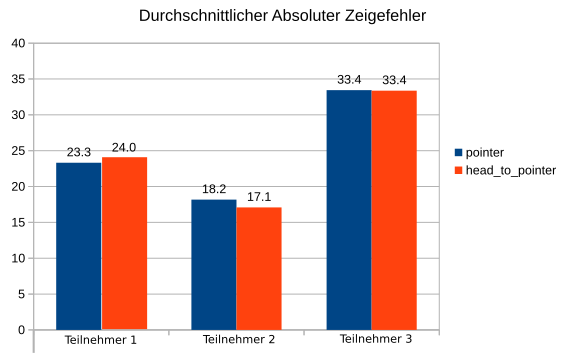
\includegraphics[width=0.8\textwidth]{images/average.png}
  \caption{Die durchschnittlichen Zeigefehler der drei Probanden.}
  \label{fig:todo}
\end{figure}

\begin{figure}[]
  \centering
  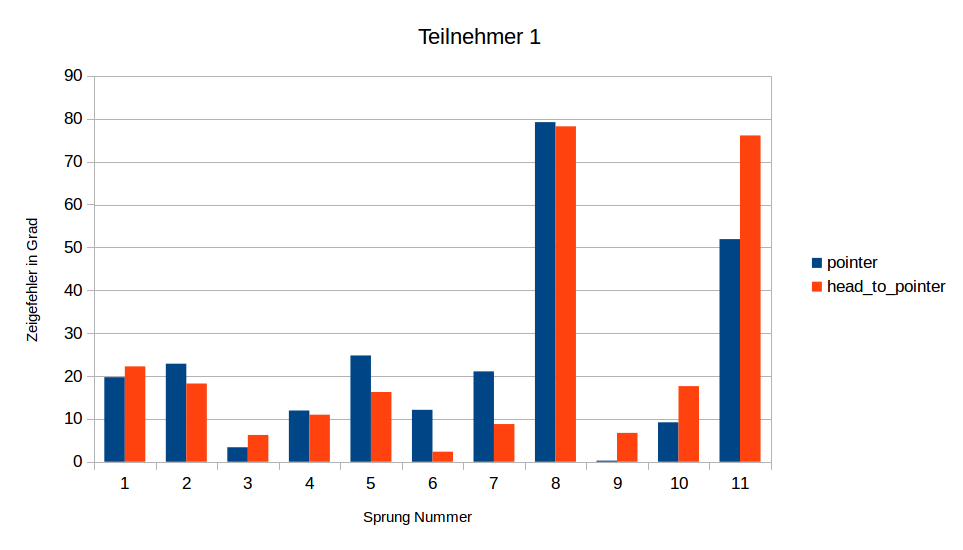
\includegraphics[width=0.8\textwidth]{images/teilnehmer1.png}
  \caption{Die Ergebnisse des ersten Teilnehmers.}
  \label{fig:todo}
\end{figure}


\begin{figure}[]
  \centering
  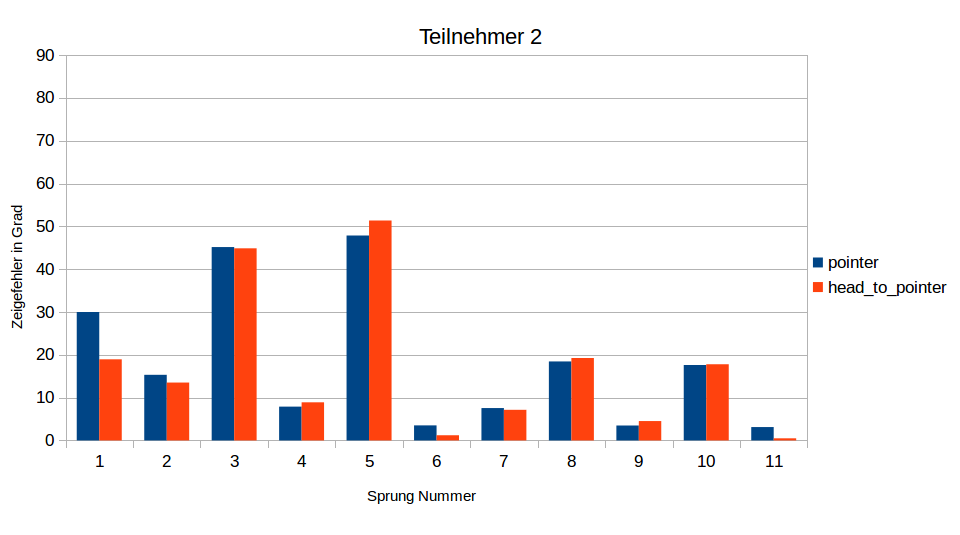
\includegraphics[width=0.8\textwidth]{images/teilnehmer2.png}
  \caption{Die Ergebnisse des zweiten Teilnehmers.}
  \label{fig:todo}
\end{figure}


\begin{figure}[]
  \centering
  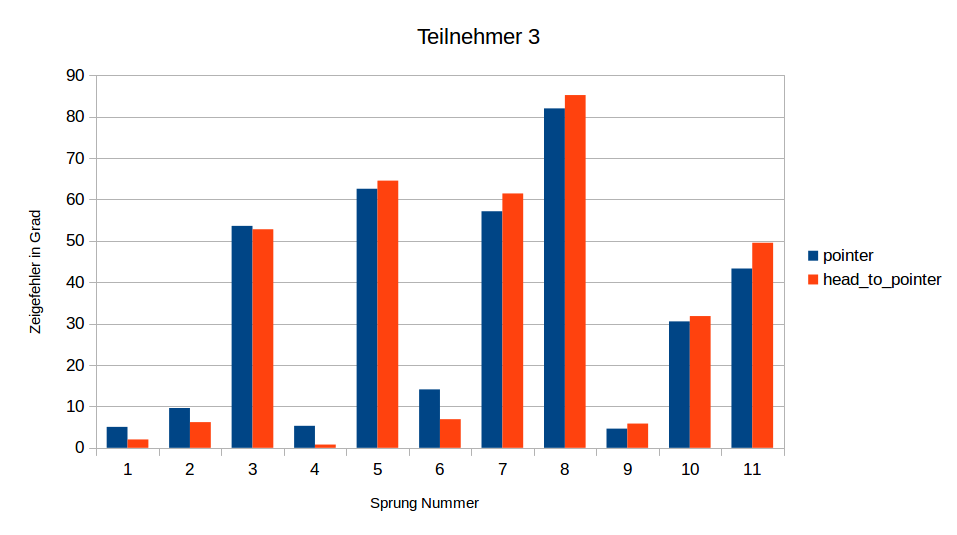
\includegraphics[width=0.8\textwidth]{images/teilnehmer3.png}
  \caption{Die Ergebnisse des dritten Teilnehmers.}
  \label{fig:todo}
\end{figure}


\begin{figure}[]
  \centering
  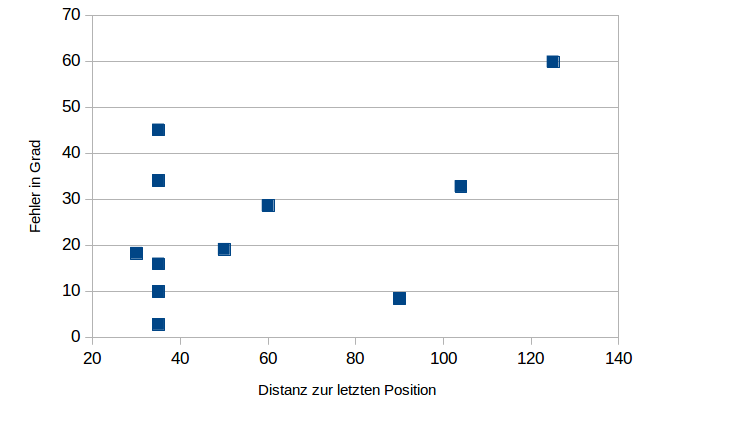
\includegraphics[width=0.8\textwidth]{images/fehlernachdistanz.png}
  \caption{Der durchschnittliche Zeigefehler aller Nutzer, geordnet nach Sprungdistanz. Es scheint keine Korrelation zwischen Sprungdistanz und Zeigefehler zu geben.}
  \label{fig:todo}
\end{figure}


\begin{figure}[]
  \centering
  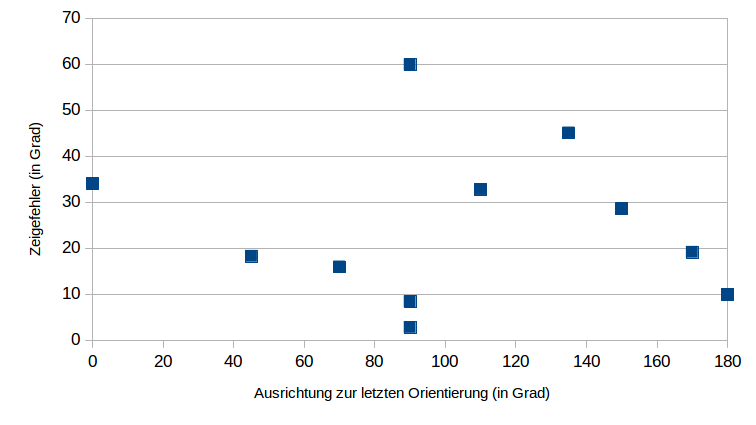
\includegraphics[width=0.8\textwidth]{images/fehlernachausrichtung.png}
  \caption{Der durchschnittliche Zeigefehler aller Nutzer, geordnet nach dem Winkel zwischen aktueller und letzter Ausrichtung. Es scheint ebenfalls keine Korrelation zwischen Orientierung vor/nach dem Sprung und dem Zeigefehler zu geben.}
  \label{fig:todo}
\end{figure}



\newpage
Auch das Einzeichnen der bereisten Orte zeigt, dass die erwarteten 80\% grundsätzlich im möglichen Bereich liegen. Dabei hängt natürlich sehr viel davon ab, wie großzügig die Bewertung vorgenommen wird. Die nachfolgenden Bilder zeigen die eingezeichneten Orte, sowie die (natürlich nachträglich eingefügten) tatsächlichen Aufenthaltsorte. Beispielhaft wurden hier für die 11 Orte jeweils ein Punkt für den grundsätzlich richtigen Ort und ein weiterer Punkt für die richtige Orientierung vergeben. Insgesamt konnten also von allen drei Nutzern 66 Punkte erreicht werden, von denen 54 letztendlich als gültig gezählt werden. Dies entspricht einem Ergebnis von ca. 82\%.


\begin{figure}[]
  \centering
  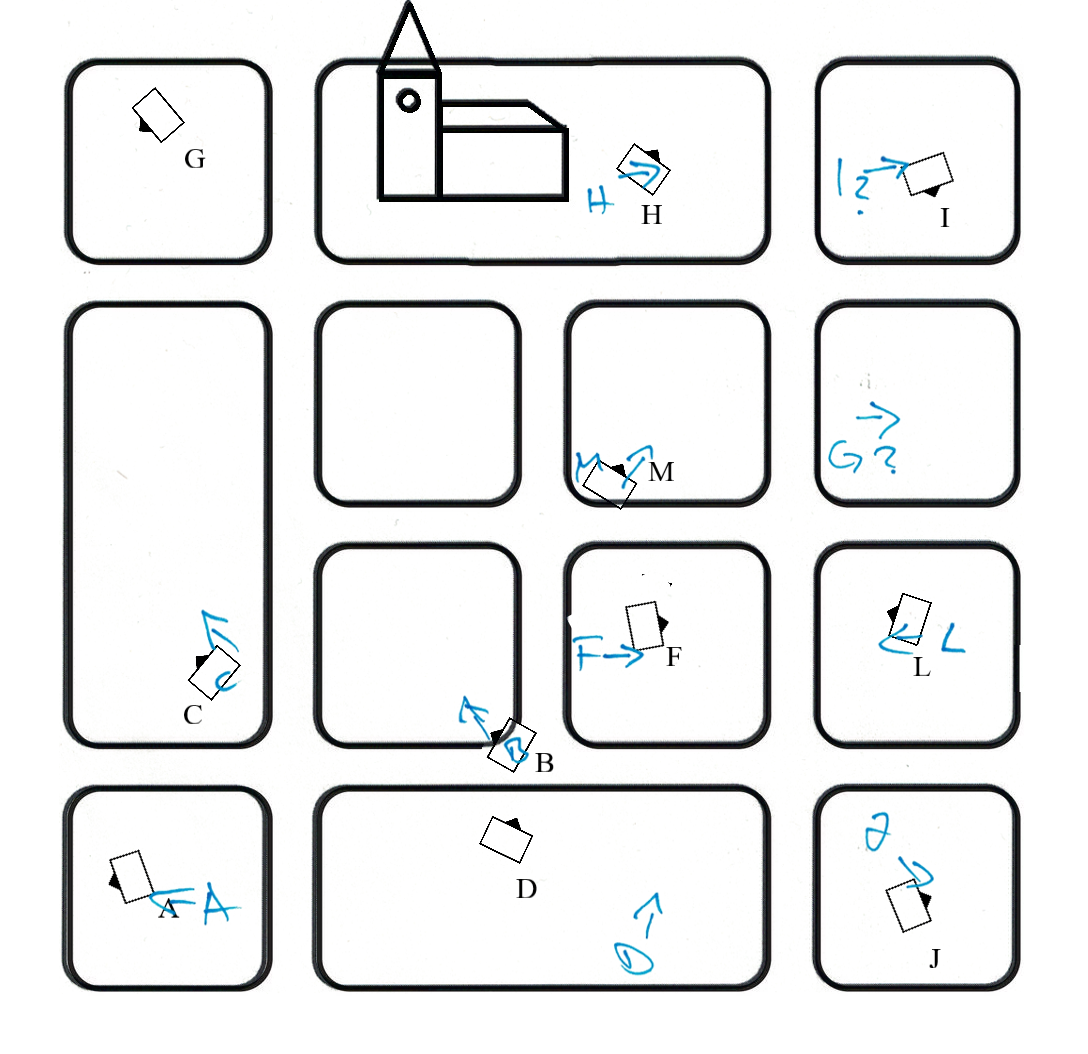
\includegraphics[width=0.8\textwidth]{images/map_full_with_curch_c.png}
  \caption{Die Karte mit den eingezeichneten Orten, Teilnehmer 1. Ergebnis: 17/22 Punkte.}
  \label{fig:todo}
\end{figure}


\begin{figure}[]
  \centering
  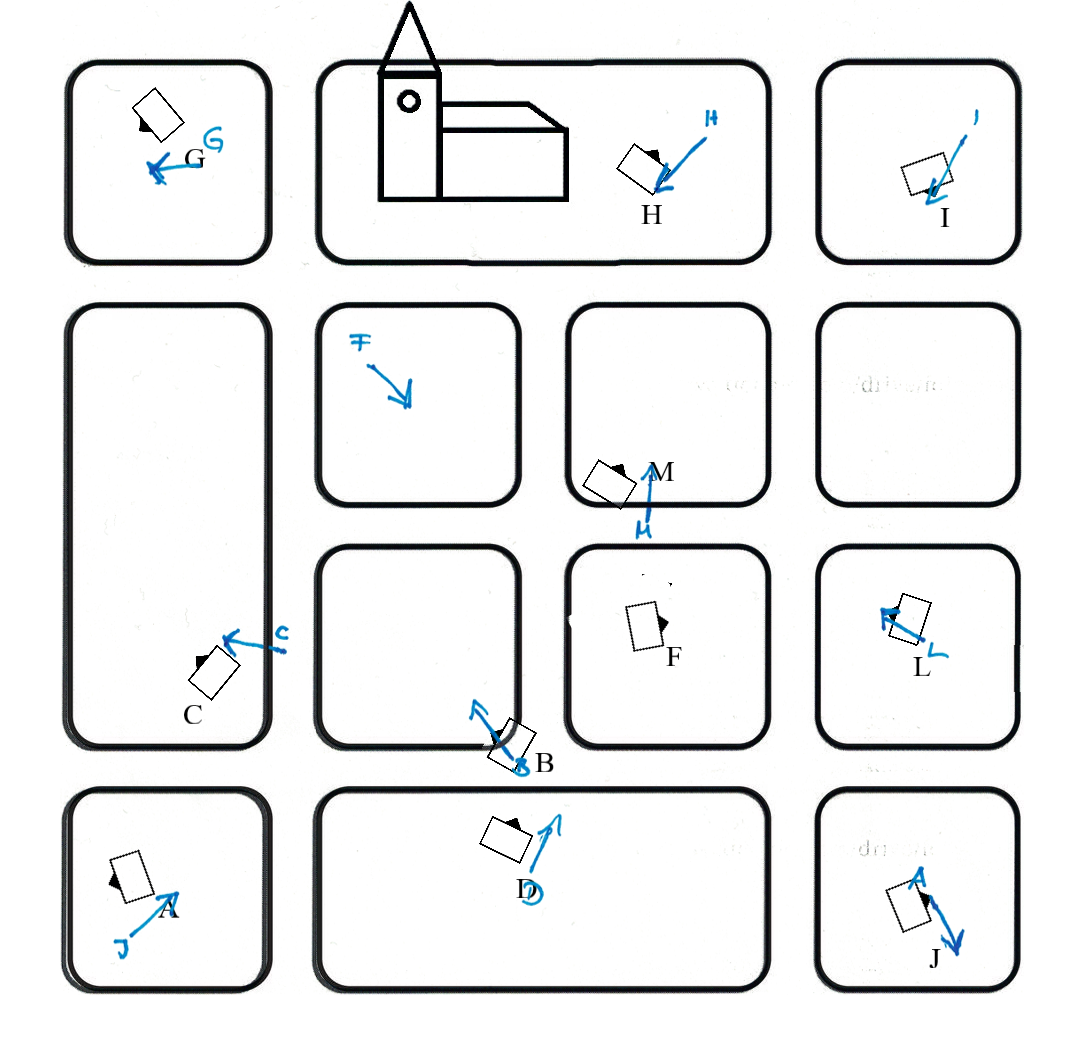
\includegraphics[width=0.8\textwidth]{images/map_full_with_curch_b.png}
  \caption{Die Karte mit den eingezeichneten Orten, Teilnehmer 2. Ergebnis: 15/22 Punkte.}
  \label{fig:todo}
\end{figure}


\begin{figure}[]
  \centering
  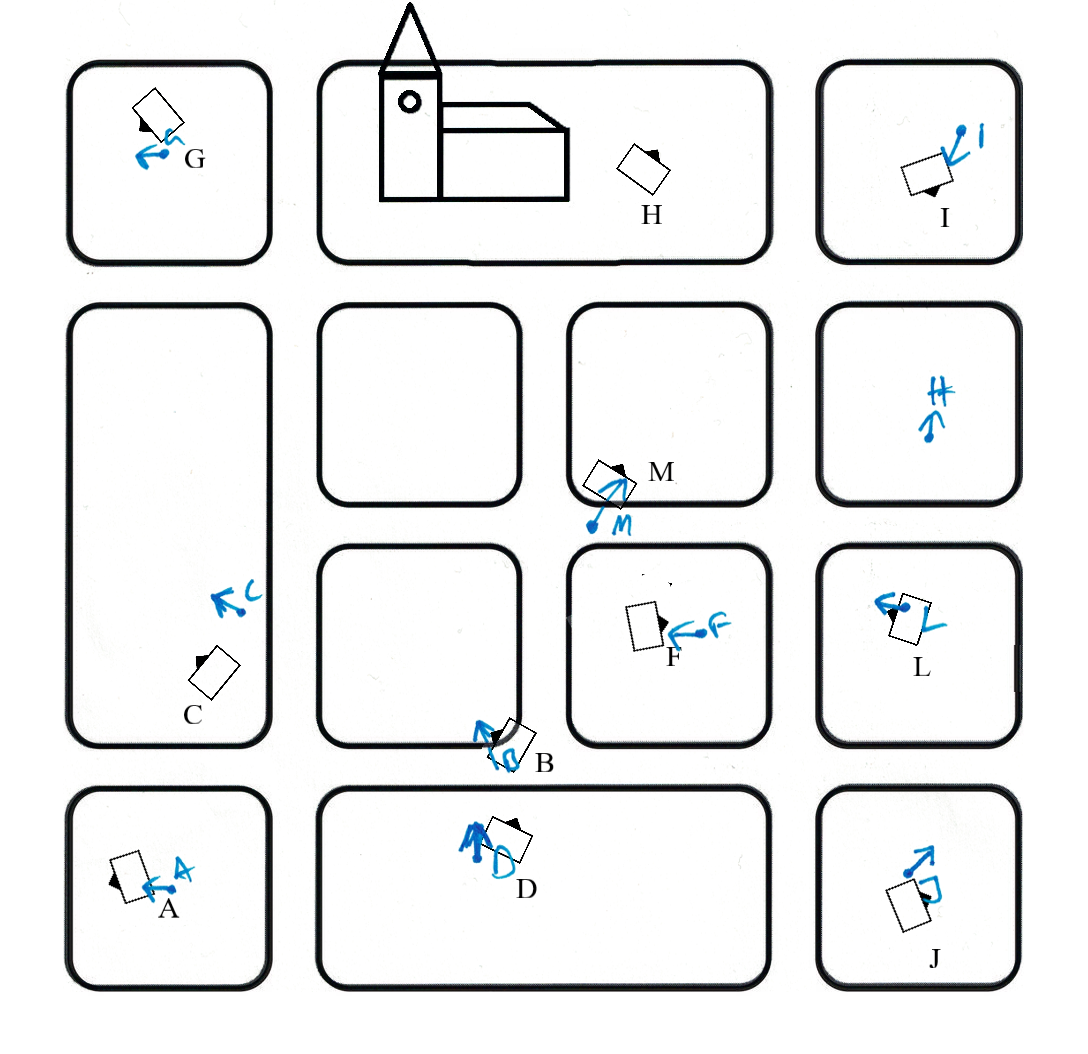
\includegraphics[width=0.8\textwidth]{images/map_full_with_curch_a.png}
  \caption{Die Karte mit den eingezeichneten Orten, Teilnehmer 3. Ergebnis: 19/22 Punkte.}
  \label{fig:todo}
\end{figure}


\subsection{Verbesserungsvorschläge}
Grundsätzlich stellte die Pilotstudie eine Minimalvariante einer tatsächlichen Studiendurchführung dar. Neben dem Durchführen des SSQ und SUS, sowie einer ausreichenden Einführung in das System gibt es Punkte, die noch berücksichtigt werden müssen.
Wichtig ist beispielsweise, dass in den Fotos keine Referenzpunkte sichtbar sein dürfen, die beim Einzeichnen in die Karte dazu führen könnten, dass der Nutzer sich an diesen und nicht an seiner Erinnerung orientiert. Weiterhin fiel auf, dass es bei der Testdurchführung in einem Fall möglich war, den zuletzt besuchten Ort direkt zu sehen (Sprung 9). Das Zeigen in diese Richtung ist dementsprechend einfach. Dieser Sprung sollte also ersetzt werden.
Bereits in der Pilotstudie wurde abgefragt, ob man sich wirklich erinnern kann, wo der letzte Aufenthaltsort war. Denn bereits in Vortest fiel auf, dass Nutzer in manchen Fällen gar keine Vorstellung haben, in welche Richtung sie zeigen sollen und sich infolgedessen an ihrem Partner orientieren. In der Auswertung einer Studie könnte man diese Ergebnisse herausrechnen oder mit einem hohen Fehler \glqq bestrafen\grqq{}.
Generell wurde darauf geachtet, dass die Sprünge eine hohe Variabilität in Distanz und Orientierung aufweisen. Dies ließe sich aber noch systematischer Klassifizieren als im Testlauf geschehen.
Was in dieser Studie nicht berücksichtigt wurde, ist die Platzierung der Nutzerplattform in der Luft. Hierbei müsste man allerdings die Berechnung des Zeigewinkels überdenken, da aktuell nur die zweidimensionale Himmelsrichtung berücksichtigt wird.
Abschließend lässt sich sagen, dass für die Evaluierung einer Interaktionstechnik das subjektive Feedback der Tester sehr wichtig ist. Im Laufe der Entwicklung hat sich gezeigt, dass alle, die die Technik nutzten recht schnell lernten, diese zu bedienen. Dennoch wäre es hier wichtig, Meinungen und Einschätzungen zu sammeln und zu berücksichtigen.

\section{Weitere Studienkonzepte}
Neben der nun vorgestellten Studiendurchführung gibt es weitere Möglichkeiten, wie sich die Technik ebenfalls evaluieren ließe. Denkbar wäre zum Beispiel ein Vergleich mit einer (skalierungsbasierten) Steeringtechnik (wie z.B. bei \cite{Dallat2018Giant}) oder dem Multiray-Jumping\cite{WeisskerMulti-RayReality}. Ebenfalls denkbar wäre eine Verhaltensstudie, bei der die Kooperation zweier oder mehr Teilnehmer bei der Benutzung dieser Technik untersucht wird, indem die Teilnehmer gefilmt werden und die gemeinsame Interaktion im Fokus steht.